\chapter{嵌入式系统开发实验}{入门}\label{ch-env}

\section{实验目的}
    了解嵌入式系统的开发环境、内核的下载和启动过程

\section{嵌入式系统开发过程}
    嵌入式系统与普通计算机系统存在很大区别,主要表现在:
\begin{itemize}\itemsep=-3pt
  \item 嵌入式系统往往不提供BIOS,因此基本输入输出系统需要程序员完成;
  \item 嵌入式系统开发缺乏友好的人机界面,为程序调试带来困难;
  \item 嵌入式系统开发能力不如通用计算机系统.通常采用交叉编译的方式,
        在通用计算机上编译嵌入式系统的程序;
  \item 嵌入式系统的存储空间有限,对程序优化要求较高.
\end{itemize}
    上述特点决定了在嵌入式系统开发中所使用的工具、方法的特殊性.

\begin{figure}[!h]
\centering
  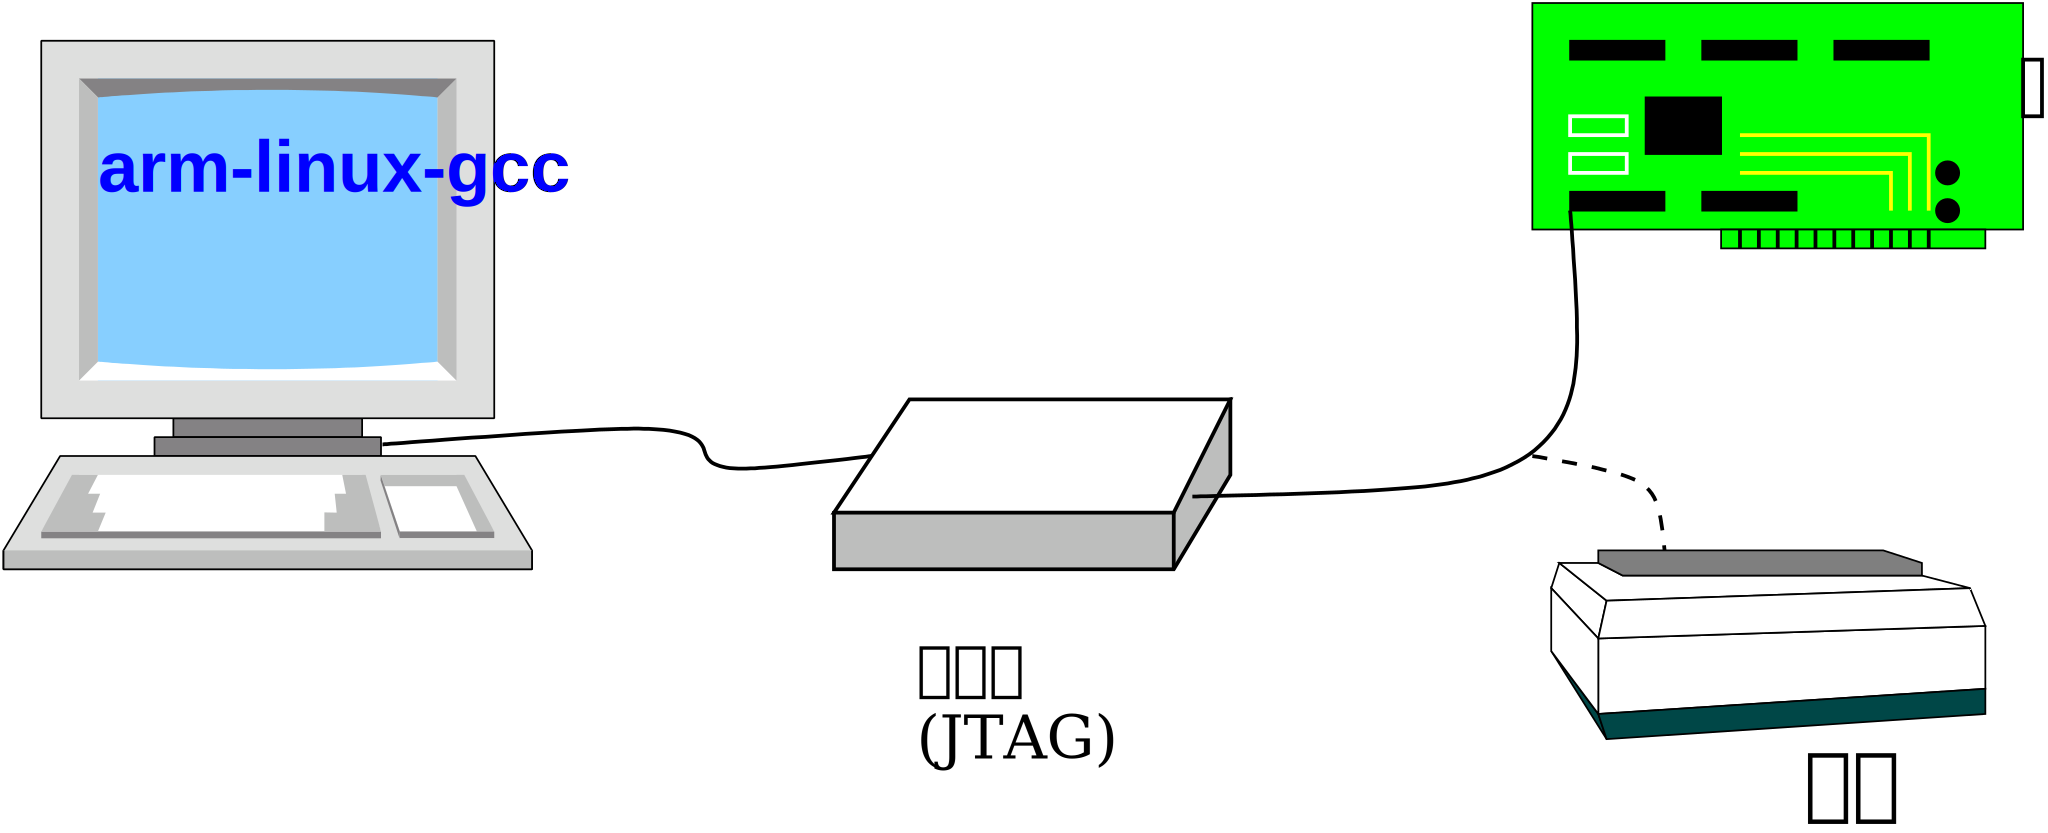
\includegraphics[width=.55\textwidth]{host-obj}
\caption{宿主机/目标机的开发模式}
\end{figure}

    本系统主要基于串行口和网口进行开发.

\subsection{bootloader}
	PC 机中的引导加载程序由 BIOS 和位于硬盘的主引导记录 MBR(Master Boot
Recorder) 中的 OS Boot Loader 一起组成.BIOS 在完成硬件检测和资源分配
后,将硬盘 MBR 中的 Boot Loader 读到系统的 RAM 中,然后将控制权交给
OS Boot Loader.Boot Loader 的主要运行任务就是将内核映像从硬盘上读到
RAM 中,然后跳转到内核的入口点去运行,也即开始启动操作系统.

	嵌入式系统中,通常并没有像 BIOS 那样的固件程序,因此整个系统的加载启动
任务完全由 bootloader 来完成.用于引导嵌入式操作系统的 bootloader 有
U-Boot、vivi、RedBoot等等.bootloader的主要作用是:
\begin{enumerate}\itemsep=-3pt
  \item 初始化硬件设备;
  \item 建立内存空间的映射图;
  \item 完成内核的加载,为内核设置启动参数.
\end{enumerate}

\subsection{bootloader程序结构框架}
	嵌入式系统中的 bootloader 的实现完全依赖于 CPU 的体系结构,因此
大多数 bootloader 都分两个阶段.依赖于 CPU 体系结构的代码,比如设备初始化
代码等,通常都放在阶段一中,且通常都用汇编语言来实现,以达到短小精悍的目的.
阶段一通常包括以下步骤:
\begin{enumerate}\itemsep=-5pt
  \item 硬件设备初始化;
  \item 拷贝Boot Loader的程序到RAM空间中;
  \item 设置好堆栈;
  \item 跳转到阶段二的c入口点.
\end{enumerate}

	阶段二则通常用c语言来实现,这样可以实现一些复杂的功能,而且代码会具有更好的可读性和可移植性.这一阶段主要包括以下步骤:
\begin{enumerate}\itemsep=-3pt
  \item 初始化本阶段要使用到的硬件设备;
  \item 系统内存映射(memory map);
  \item 将kernel映像和根文件系统映像从Flash读到RAM空间中; 
  \item 为内核设置启动参数;
  \item 调用内核.
\end{enumerate}

\subsection{串口设置(minicom)}
    多数嵌入式系统都通过异步串行接口(UART)进行初级引导.这种通信方式是将
字符一位一位地传送,一般是先低位、后高位.因此,采用串行方式,双方最少可以
只用一对连线便可实现全双工通信.字符与字符之间的同步靠每个字框的起始位协调,
而不需要双方的时钟频率严格一致,因此实现比较容易.

    RS-232C 是通用异步串行接口中最常用的标准.它原是美国电子工业协会推荐的
标准(EIA RS-232C, Electronics Industrial Association Recommended
Standard),后被世界各国所接受并应用到计算机的I/O接口中.个人计算机系统中常
使用25针或9针接插件(DB-25/DB-9)连接.例如,DB-25按图\ref{pc-serial}
定义了接口信号.

\begin{figure}
\centering
\begin{tikzpicture}[
	point/.style={coordinate},>=stealth',thick,draw=black!50,align=left,
	block/.style={rectangle, draw=none, text width=9em,align=left,
	text height=3ex},
	line/.style={draw, thick, -latex',shorten >=2pt},
	hv path/.style={to path={-| (\tikztotarget)}},
	vh path/.style={to path={|- (\tikztotarget)}}]

	\fontsize{10}{20} \selectfont\tt
	\matrix[column sep=6mm] {
	\node[block]{保护地(接外壳)};   &\node(a1)   {1}; & & &\node(b1)   {1};&
		&\node(c1)   {1}; & & &\node(d1)   {1};\\
	\node[block]{数据发送 TxD};     &\node(a2)   {2}; & & &\node(b2)   {2};&
		&\node(c2)   {2}; & & &\node(d2)   {2};\\
	\node[block]{数据接受 RxD};     &\node(a3)   {3}; & & &\node(b3)   {3};&
		&\node(c3)   {3}; & & &\node(d3)   {3};\\
	\node[block]{信号地};           &\node(a7)   {7}; & & &\node(b7)   {7};&
		&\node(c7)   {7}; & & &\node(d7)   {7};\\
	\node[block]{请求发送 RTS};     &\node(a4)   {4}; & & &\node(b4)   {4};&
		&\node(c4)   {4}; & & &\node(d4)   {4};\\
	\node[block]{清除发送 CTS};     &\node(a5)   {5}; & & &\node(b5)   {5};&
		&\node(c5)   {5}; & & &\node(d5)   {5};\\
	\node[block]{载波检测 DCD};     &\node(a8)   {8}; & & &\node(b8)   {8};&
		&\node(c8)   {8}; & & &\node(d8)   {8};\\
	\node[block]{数据装置就绪 DSR}; &\node(a6)   {6}; & & &\node(b6)   {6};&
		&\node(c6)   {6}; & & &\node(d6)   {6};\\
	\node[block]{振铃指示 RI};      &\node(a22)  {22};& & &\node(b22)  {22};&
		&\node(c22)  {22};& & &\node(d22)  {22};\\
	\node[block]{数据终端就绪 DTR}; &\node(a20)  {20};& & &\node(b20)  {20};&
		&\node(c20)  {20};& & &\node(d20)  {20};\\
	 & & & \node{三线式};& & & &\node{七线式};& & \\
	};
	\node (e2) [right=of a2] {};
	\draw [dashed] (a1) -- (b1);
	\draw [->] (a2) -- ++(8mm,0) -- ($(b3)-(8mm,0)$) --(b3);
	\draw [<-] (a3) -- ++(8mm,0) -- ($(b2)-(8mm,0)$)-- (b2);
	\draw [-] (a7) -- (b7);
	\draw [->] (a4) -- ++(8mm,0) |- (a5);
	\draw [->] (a4) -- ++(8mm,0) |- (a8);
	\draw [->] (b4) -- ++(-8mm,0) |- (b5);
	\draw [->] (b4) -- ++(-8mm,0) |- (b8);
	\draw [->] (a20) -- ++(8mm,0) |- (a22);
	\draw [->] (a20) -- ++(8mm,0) |- (a6);
	\draw [->] (b20) -- ++(-8mm,0) |- (b22);
	\draw [->] (b20) -- ++(-8mm,0) |- (b6);

	\draw [dashed] (c1) -- (d1);
	\draw [->] (c2) -- ++(8mm,0) -- ($(d3)-(8mm,0)$) --(d3);
	\draw [<-] (c3) -- ++(8mm,0) -- ($(d2)-(8mm,0)$)-- (d2);
	\draw [-] (c7) -- (d7);
	\draw [->] (c4) -- ++(8mm,0) |- (c5);
	\draw [->] (c5) ++(8mm,0) -- ($(d8)-(8mm,0)$) -- (d8);
	\draw [->] (d4) -- ++(-8mm,0) |- (d5);
	\draw [->] (d5) ++(-8mm,0) -- ($(c8)+(8mm,0)$) -- (c8);
	\draw [->] (c6) -- ++(8mm,0) |- (c22);
	\draw [->] (d6) -- ++(-8mm,0) |- (d22);
	\draw [-] (c22) ++(8mm,0) --($(d20)-(8mm,0)$)-- (d20);
	\draw [-] (d22) ++(-8mm,0) --($(c20)+(8mm,0)$) -- (c20);

\end{tikzpicture}
\caption{PC机串口引脚信号}\label{pc-serial}
\end{figure}


\iffalse
\fontsize{10}{20} \selectfont \kai\centering
\begin{tabular}{lrp{3cm}lcrp{3cm}l}
  保护地(接外壳)   &\rnode{a1}{1}& &\rnode{b1}{1}&
                   &\rnode{c1}{1}& &\rnode{d1}{1}\\
  数据发送 TxD     &\rnode{a2}{2}& &\rnode{b2}{2}&
                   &\rnode{c2}{2}& &\rnode{d2}{2}\\
  数据接受 RxD     &\rnode{a3}{3}& &\rnode{b3}{3}&
                   &\rnode{c3}{3}& &\rnode{d3}{3}\\
  信号地           &\rnode{a7}{7}& &\rnode{b7}{7}&
                   &\rnode{c7}{7}& &\rnode{d7}{7}\\
  请求发送 RTS     &\rnode{a4}{4}& &\rnode{b4}{4}&
                   &\rnode{c4}{4}& &\rnode{d4}{4}\\
  清除发送 CTS     &\rnode{a5}{5}& &\rnode{b5}{5}&
                   &\rnode{c5}{5}& &\rnode{d5}{5}\\
  载波检测 DCD     &\rnode{a8}{8}& &\rnode{b8}{8}&
                   &\rnode{c8}{8}& &\rnode{d8}{8}\\
  数据装置就绪 DSR &\rnode{a6}{6}& &\rnode{b6}{6}&
                   &\rnode{c6}{6}& &\rnode{d6}{6}\\
  振铃指示 RI      &\rnode{a22}{22}& &\rnode{b22}{22}&
                   &\rnode{c22}{22}& &\rnode{d22}{22}\\
  数据终端就绪 DTR &\rnode{a20}{20}& &\rnode{b20}{20}&
                   &\rnode{c20}{20}& &\rnode{d20}{20}\\
                   &    & 三线式 & & & & 七线式 &
\end{tabular}
\ncline[linestyle=dashed]{-}{a1}{b1}
\ncdiag[angleA=0,angleB=180,arm=20pt]{->}{a2}{b3}
\ncdiag[angleA=180,angleB=0,arm=20pt]{->}{b2}{a3}
\ncline[]{-}{a7}{b7}
\ncline[linestyle=dashed]{-}{c1}{d1}
\ncdiag[angleA=0,angleB=180,arm=20pt]{->}{c2}{d3}
\ncdiag[angleA=180,angleB=0,arm=20pt]{->}{d2}{c3}
\ncline[]{-}{c7}{d7}
\ncdiag[angleA=0,angleB=0,arm=20pt]{->}{a4}{a8}
\ncdiag[angleA=0,angleB=0,arm=20pt]{->}{a4}{a5}
\ncdiag[angleA=0,angleB=0,arm=20pt]{->}{a20}{a6}
\ncdiag[angleA=0,angleB=0,arm=20pt]{->}{a20}{a22}
\ncdiag[angleA=180,angleB=180,arm=20pt]{->}{b4}{b8}
\ncdiag[angleA=180,angleB=180,arm=20pt]{->}{b4}{b5}
\ncdiag[angleA=180,angleB=180,arm=20pt]{->}{b20}{b6}
\ncdiag[angleA=180,angleB=180,arm=20pt]{->}{b20}{b22}
\ncdiag[angleA=0,angleB=0,arm=20pt]{->}{c4}{c5}
\ncdiag[angleA=0,angleB=180,arm=20pt]{->}{c5}{d8}
\ncdiag[angleA=180,angleB=180,arm=20pt]{->}{d4}{d5}
\ncdiag[angleA=180,angleB=0,arm=20pt]{->}{d5}{c8}
\ncdiag[angleA=0,angleB=0,arm=20pt]{->}{c6}{c22}
\ncdiag[angleA=180,angleB=0,arm=20pt]{->}{d20}{c22}
\ncdiag[angleA=180,angleB=180,arm=20pt]{->}{d6}{d22}
\ncdiag[angleA=0,angleB=180,arm=20pt]{->}{c20}{d22}
\fi

	Linux系统用 minicom 软件实现串口通信.

\begin{figure}
\centering \fontsize{10}{10}\selectfont
\begin{boxedminipage}{.96\textwidth}
\begin{verbatim}
Welcome to minicom 2.4

OPTIONS: I18n
Compiled on Jan 25 2010, 06:49:09.
Port /dev/ttyS0

Press CTRL-A Z for help on special keys

            +-----[configuration]------+
            | Filenames and paths      |
            | File transfer protocols  |
            | Serial port setup        |
            | Modem and dialing        |
            | Screen and keyboard      |
            | Save setup as dfl        |
            | Save setup as..          |
            | Exit                     |
            +--------------------------+




 CTRL-A Z for help |115200 8N1 | NOR | Minicom 2.4    | VT102 |      Offline
\end{verbatim}
\end{boxedminipage}
\caption{minicom界面}
\end{figure}

    运行 minicom, \^{}A--o,进入 minicom 设置界面\footnote{\^{}A是
minicom 的控制键,可以激活其他功能设置,例如\^{}A--z 调出全部功能菜单,
\^{}A--x 退出 minicom.也可以在minicom启动时加上选项``--s''直接进入设置界面}.
在 Serial port setup 项上修改下述设置:
\begin{itemize}\itemsep=-3pt
  \item A --- ``Serial Device'',串口通信口的选择.如果串口线接在PC机的串口1
		上,则为 /dev/ttyS0,如果连接在串口2上,则为 /dev/ttyS1,依此类推.
  \item E --- ``Bps/Par/Bits'',串口参数的设置.设置通信波特率、数据位、
		奇偶校验位和停止位.本实验平台要求把波特率设置为115200bps,数据位
		设为8位,无奇偶校验,一个停止位;
  \item F --- ``Hardware Flow Control''、G --- ``Software Flow Control'',
		数据流的控制选择.按``F''或``G''键完成硬件软件流控制切换(即
		``Yes''与``No''之间的切换).本实验系统都设置为``No''.
\end{itemize}

	配置完成后,选择``Save setup as dfl''保存配置,并返回 minicom 的主界面.
以后使用不再需要每次设置.

	给开发板加电,这时可以在 minicom 主界面上看到开发板的启动信息.在短时间内
(时间可通过bootloader命令设置)通过键盘干预, 将停止加载内核, 进入人机交互方式,
出现提示符 ``x210 \#''.``help''命令可列出所有u-boot的命令;如需了解具体某个
命令的使用, 可用``help + 命令''的方式.

	以下列出本实验常用的命令:
\begin{itemize}
  \item setenv: 设置环境变量.主要的环境变量有:
  \begin{itemize}
    \item ipaddr, serverip, gatewayip,本机和服务器的IP地址,网关
    \item bootargs, 启动参数,一般包括监控端口、内核启动参数,加载文件系统等,
		如 setenv bootargs console=ttySAC2,115200 root=/dev/mtdblock2 rw
             rootfstype=yaffs2 init=/linuxrc, 表示用串口设备ttySAC2作为
		终端,波特率115200bps,根文件系统在eMMC卡(或FLASH)的第二分区,读写
		允许,yaffs2文件系统, 内核启动后执行根目录下的 linuxrc 命令.
	\item bootcmd, 启动命令,上电后或者执行 boot 命令后调用.如
		setenv bootcmd 'movi read kernel 0xc0008000;bootm 0xc0008000'
		表示将 eMMC 卡的 kernel 分区读到内存以 0xc0008000起始的地址中,然后
		从0xc0008000处开始运行.
  \end{itemize}
  \item tftp, tftp 命令,如 tftp 0xc0008000 zImage,将 tftp 服务器目录中的
        文件 zImage 通过 tftp 协议读入内存 0xc0008000 起始处.
  \item saveenv 保存环境变量设置.未经保存的环境变量,重启后将恢复原状.
\end{itemize}


\subsection{tftp}
    tftp 是基于UDP协议的简单文件传输协议.目标板作为客户机,bootloader 默认
采用 tftp 协议.主机安装 tftp-server,作为 tftp 服务器.Linux系统的 tftp
服务由超级服务器 xinetd 管理.安装 tftp-server 后,/etc/xinetd.d/tftp
中大致是如下内容:
\footnote{主机的不同发行版、不同的软件,使用方法和配置文件有所不同, 关键要
了解服务的目的、目录、权限及启动方式; 下面的NFS服务亦然}

\begin{verbatim}
  service tftp
  { 
      socket_type = dgram
      protocol  = udp
      wait = yes
      user = root
      server = /usr/sbin/in.tftpd
      server_args     = -c -s /tftpboot
      disable = yes
      per_source = 11
      cps = 100 2
  }
\end{verbatim}

    将``disable''的选项改为``no'',关闭防火墙,再用如下命令重启tftp服务:

\begin{boxedminipage}{.9\textwidth}
\begin{verbatim}
  # /etc/rc.d/init.d/xinetd restart
\end{verbatim}
\end{boxedminipage}

	tftp的配置文件里表明,tftp 服务的主目录是 /tftpboot,因此只有在这个
目录下面的文件才可以通过 tftp 进行下载.我们需要 bootloader 从服务器上下载
内核及文件系统.为实现这个目的,需要配置客户端(目标机)的网络 IP 地址,
使其和主机处于同一网段,并注意不要和其他系统(包括主机和目标机)的IP发生冲突.
u-boot中, 用``setenv ipaddr''和``setenv serverip'' 分别设置本机和 tftp
服务器的IP地址.

\subsection{NFS服务器架设}
      NFS 是 Network File System 的缩写.NFS 是由 Sun 公司开发并发展起来的
一项用于在不同机器、不同操作系统之间通过网络共享文件的服务系统.nfs-server
也可以看作是一个文件服务器,它可以让 PC 通过网络将远端的 nfs server 共享
出来的档案挂载到自己的系统中.在客户端看来,使用 NFS 的远端文件就像是在
使用本地文件一样.

    NFS 协议从诞生到现在为止,已经有多个版本,如 NFS V2(rfc1094)、NFS
V3(rfc1813)、NFS V4(rfc3010)等.

    NFS 涉及到 portmap 和 NFS 两个服务.需要在主机打开这两个服务:

\begin{boxedminipage}{.9\textwidth}
\begin{verbatim}
  # chkconfig nfs on
  # chkconfig portmap on
  # service nfs restart
  # service portmap restart
\end{verbatim}
\end{boxedminipage}

服务器的共享目录和权限在 /etc/exports 中设定.下面是这个文件的样例:

\begin{boxedminipage}{.9\textwidth}
\begin{verbatim}
  # this is a sample
  # /etc/exports
  /opt  192.168.1.*(rw,no_root_squash)
\end{verbatim}
\end{boxedminipage}

使用如下命令使修改生效:

\begin{boxedminipage}{.9\textwidth}
\begin{verbatim}
  # exportfs -a
\end{verbatim}
\end{boxedminipage}

    目标板上的 Linux 启动后, BusyBox可以提供操作系统人机交互的基本功能.
如果需要配置网络, 使用 ifconfig, 和主机的用法相同:

\begin{boxedminipage}{.9\textwidth}
\begin{verbatim}
  # ifconfig eth0 192.168.1.xx
\end{verbatim}
\end{boxedminipage}

如果内核和BusyBox都支持 NFS, 可以用 mount 命令将主机的 /opt 目录挂在/mnt 
目录下(设主机的IP为192.168.1.100):

\begin{boxedminipage}{.9\textwidth}
\begin{verbatim}
  # mount 192.168.1.100:/opt /mnt -o nolock -o proto=tcp
\end{verbatim}
\end{boxedminipage}

 这样当访问目标板的 /mnt 目录时,访问的就是服务器上的 /opt 目录的内容.

\subsection{使用gcc、g++等工具编译应用程序}
\begin{enumerate}\itemsep=-3pt
  \item 编写一个简单的独立程序;
  \item 使用交叉编译工具编译;
  \item 将编译生成的可执行程序 hello 拷贝到 NFS 共享目录下,在目标板上
		运行该程序.

        如果不能运行, 请在gcc编译选项中加上 -{}-static
\end{enumerate}

\section{实验报告要求}
    归纳总结嵌入式系统下软件开发的一般流程
